\paragraph{curve-assert-valid}

\subparagraph{Target}
Check the point is on the curve $y^2 = x^3 + ax + b$.

\subparagraph{Process layout}
See \figref{fig:curve-assert-valid-layout}.
\begin{figure}[!ht]
    \centering
    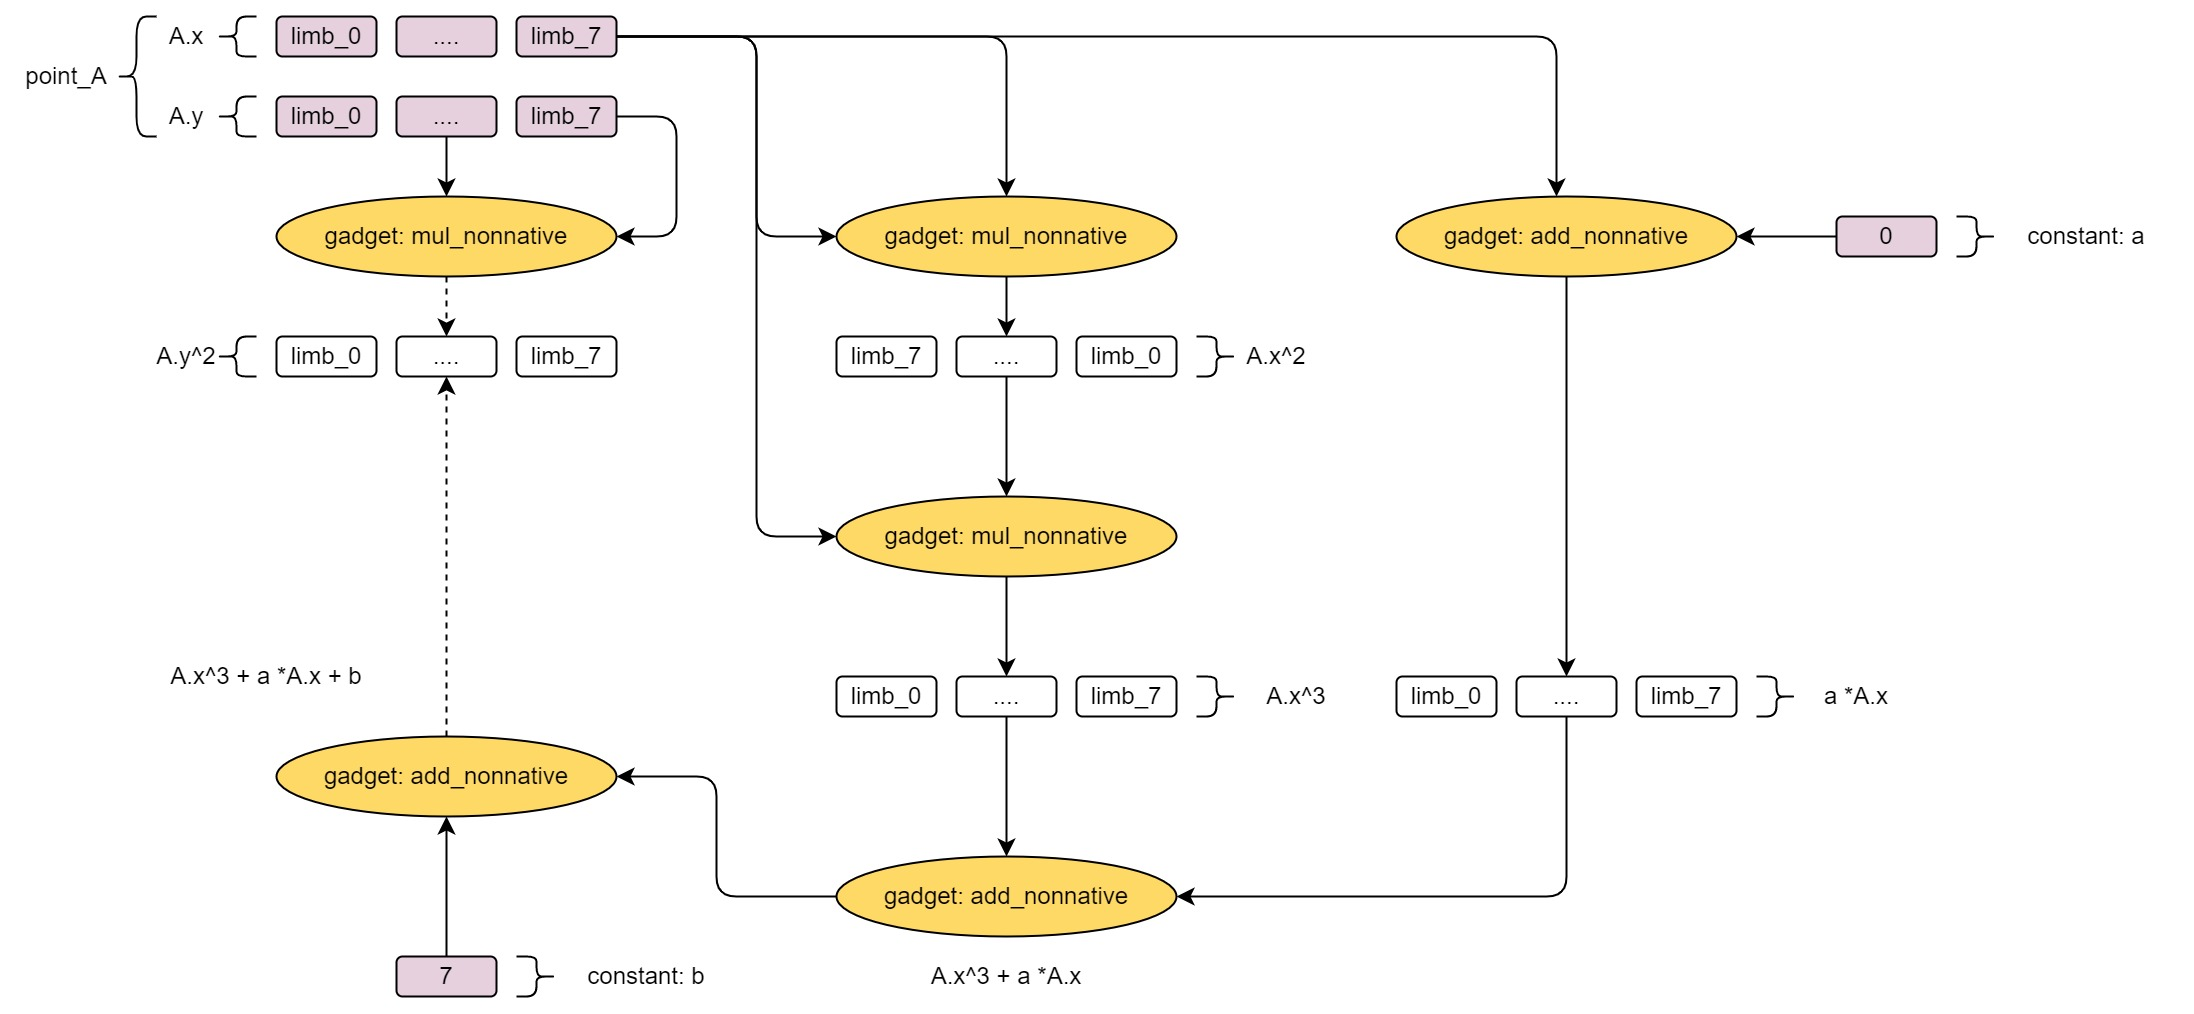
\includegraphics[width=0.6\textwidth]{curve-assert-valid-layout.jpg}
    \caption{curve-assert valid layout}
    \label{fig:curve-assert-valid-layout}
\end{figure}

\subparagraph{Constraints info and costs}
\begin{itemize}
    \item gadget-add-nonnative num: 3
    \item gadget-mul-nonnative num: 3
    \item gate type num: 13
        \begin{itemize}
            \item 8: U32AddManyGate\{2,3,5,7,9,11,13,15\}
            \item 1: ComparisonGate
            \item 1: ArithmeticGate
            \item 1: U32ArithmeticGate
            \item 2: U32RangeCheckGate\{0,8\}
        \end{itemize}
\end{itemize}
